\documentclass[aspectratio=169]{beamer}

\usetheme{Boadilla}
\usefonttheme{professionalfonts}
\setbeamertemplate{navigation symbols}{}
\setbeamertemplate{itemize items}[circle]
\setbeamertemplate{enumerate items}[default]
\setbeamertemplate{headline}{}

\usepackage[utf8]{inputenc}
\usepackage[T1]{fontenc}
\usepackage{lmodern}
\usepackage{amsmath}
\usepackage{booktabs}
\usepackage{tabularx}
\usepackage{array}
\usepackage{hyperref}
\usepackage[strings]{underscore}
\usepackage{listings}
\usepackage{tikz}
\usetikzlibrary{arrows.meta,positioning,fit,calc,shapes.geometric}
\usepackage{xcolor}

\definecolor{courseblue}{HTML}{12355B}
\definecolor{coursegold}{HTML}{C98A2E}
\definecolor{courseice}{HTML}{EEF3F8}
\definecolor{coursegreen}{HTML}{2F6B4F}
\definecolor{coursegray}{HTML}{4B5563}
\definecolor{codebg}{HTML}{F7F9FC}
\definecolor{codecomment}{HTML}{5E6C84}
\definecolor{codestring}{HTML}{0B6E4F}

\setbeamercolor{palette primary}{bg=courseblue,fg=white}
\setbeamercolor{palette secondary}{bg=coursegold,fg=white}
\setbeamercolor{palette tertiary}{bg=courseblue,fg=white}
\setbeamercolor{palette quaternary}{bg=coursegold,fg=white}
\setbeamercolor{structure}{fg=courseblue}
\setbeamercolor{frametitle}{bg=courseice,fg=courseblue}
\setbeamercolor{title}{fg=courseblue}
\setbeamercolor{block title}{bg=courseblue,fg=white}
\setbeamercolor{block body}{bg=courseice,fg=black}
\setbeamercolor{normal text}{fg=black,bg=white}
\setbeamercolor{alerted text}{fg=coursegold}

\setbeamerfont{footline}{size=\scriptsize}

\setbeamertemplate{footline}{
  \leavevmode
  \hbox{
    \begin{beamercolorbox}[wd=.33\paperwidth,ht=2.8ex,dp=1.2ex,leftskip=0.8em]{palette primary}%
      University of Trieste
    \end{beamercolorbox}%
    \begin{beamercolorbox}[wd=.49\paperwidth,ht=2.8ex,dp=1.2ex,center]{palette tertiary}%
      \coursename{} \textbar{} \coursecode
    \end{beamercolorbox}%
    \begin{beamercolorbox}[wd=.18\paperwidth,ht=2.8ex,dp=1.2ex,rightskip=0.8em plus1fil]{palette secondary}%
      \insertframenumber{} / \inserttotalframenumber
    \end{beamercolorbox}%
  }
}

\hypersetup{
  colorlinks=true,
  linkcolor=courseblue,
  urlcolor=coursegreen
}

\lstdefinestyle{coursepython}{
  language=Python,
  basicstyle=\ttfamily\footnotesize,
  keywordstyle=\color{courseblue}\bfseries,
  commentstyle=\color{codecomment}\itshape,
  stringstyle=\color{codestring},
  showstringspaces=false,
  columns=fullflexible,
  keepspaces=true,
  frame=single,
  framerule=0.6pt,
  rulecolor=\color{courseblue},
  backgroundcolor=\color{codebg},
  xleftmargin=0.4em,
  xrightmargin=0.4em,
  aboveskip=0.4em,
  belowskip=0.2em
}

\newcommand{\coursename}{Data-driven Systems Engineering}
\newcommand{\coursecode}{440MI / 305SM}
\newcommand{\coursefooter}{}

\newcommand{\learninggoals}[1]{
  \begin{block}{Learning goals}
  #1
  \end{block}
}

\newcommand{\repoactivity}[1]{
  \begin{block}{Repo activity}
  #1
  \end{block}
}

\newcommand{\readinglist}[1]{
  \begin{block}{Papers and materials}
  {\footnotesize #1}
  \end{block}
}

\newcommand{\coursecontextframe}[5]{
  \begin{frame}{Course Map and Running Cases}
  \centering
  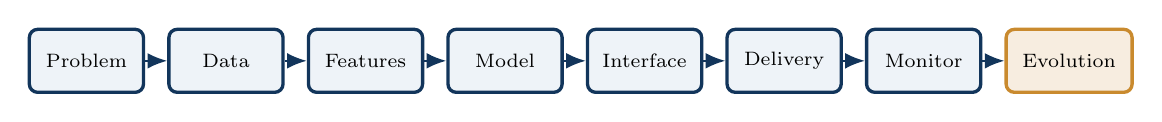
\begin{tikzpicture}[node distance=0.28cm]
  \node[flowbox, minimum width=1.45cm, minimum height=0.8cm] (problem) {\scriptsize Problem};
  \node[flowbox, minimum width=1.45cm, minimum height=0.8cm, right=of problem] (data) {\scriptsize Data};
  \node[flowbox, minimum width=1.45cm, minimum height=0.8cm, right=of data] (features) {\scriptsize Features};
  \node[flowbox, minimum width=1.45cm, minimum height=0.8cm, right=of features] (model) {\scriptsize Model};
  \node[flowbox, minimum width=1.45cm, minimum height=0.8cm, right=of model] (interface) {\scriptsize Interface};
  \node[flowbox, minimum width=1.45cm, minimum height=0.8cm, right=of interface] (delivery) {\scriptsize Delivery};
  \node[flowbox, minimum width=1.45cm, minimum height=0.8cm, right=of delivery] (monitor) {\scriptsize Monitor};
  \node[accentbox, minimum width=1.6cm, minimum height=0.8cm, right=of monitor] (evolution) {\scriptsize Evolution};
  \foreach \a/\b in {problem/data,data/features,features/model,model/interface,interface/delivery,delivery/monitor,monitor/evolution} {
    \draw[arrow] (\a) -- (\b);
  }
  \end{tikzpicture}

  \vspace{0.5em}
  \begin{block}{Today in the course}
  \textbf{Focus:} #1

  \textbf{Bridge:} #2
  \end{block}

  \begin{columns}[T]
  \column{0.48\textwidth}
  \begin{block}{Fraud case}
  {\footnotesize #3}
  \end{block}
  \column{0.48\textwidth}
  \begin{block}{Pasteurization case}
  {\footnotesize #4}
  \end{block}
  \end{columns}

  \vspace{0.3em}
  {\footnotesize \textbf{Course thread:} #5}
  \coursefooter
  \end{frame}
}

\newcommand{\classclosingframe}[4]{
  \begin{frame}{From This Class to the Next}
  \begin{block}{What stays with us}
  #1
  \end{block}

  \begin{columns}[T]
  \column{0.48\textwidth}
  \begin{block}{Project use}
  {\footnotesize #2}
  \end{block}
  \column{0.48\textwidth}
  \begin{block}{Next connection}
  {\footnotesize #3}
  \end{block}
  \end{columns}

  \vspace{0.3em}
  {\footnotesize \textbf{Course thread:} #4}
  \coursefooter
  \end{frame}
}

\tikzset{
  flowbox/.style={
    rounded corners=3pt,
    draw=courseblue,
    fill=courseice,
    very thick,
    minimum width=2.2cm,
    minimum height=0.9cm,
    align=center,
    font=\small
  },
  accentbox/.style={
    rounded corners=3pt,
    draw=coursegold,
    fill=coursegold!15,
    very thick,
    minimum width=2.2cm,
    minimum height=0.9cm,
    align=center,
    font=\small
  },
  arrow/.style={
    -{Latex[length=2.5mm,width=2mm]},
    thick,
    draw=courseblue
  }
}


\title{Class 1: Course Introduction, MLOps, and Agile AI}
\author{\coursename}
\date{}

\begin{document}

\frame{\titlepage \coursefooter}

\begin{frame}{Agenda}
\begin{itemize}
\item Course positioning: what ``data-driven systems engineering'' means in practice.
\item Why ML projects fail when they stop at the notebook.
\item The course technology stack: Python, Jupyter, pandas, scikit-learn, Flask, Streamlit, River, Docker, Jenkins, GitHub Actions.
\item Agile AI: how to structure work when data, labels, and requirements all move.
\item Running cases from this repository: fraud detection and pasteurization monitoring.
\end{itemize}
\coursefooter
\end{frame}

\begin{frame}{Why this course exists}
\learninggoals{
\begin{itemize}
\item Connect data analysis, software engineering, and operations in one engineering workflow.
\item Move from notebook-level experimentation to deployable and monitorable systems.
\item Understand what each tool in the stack is for and when not to use it.
\item Learn to discuss ML systems as socio-technical systems, not only as models.
\end{itemize}
}
\coursefooter
\end{frame}

\coursecontextframe
{End-to-end lifecycle thinking for data-driven systems.}
{We start from problem framing and follow the path all the way to deployment, monitoring, and evolution.}
{Fraud detection becomes a full service: data understanding, feature design, scoring API, release process, and monitoring.}
{Pasteurization becomes a monitoring system: synthetic sensors, forecasting or alerting logic, dashboard views, and drift-aware operation.}
{This class defines the vocabulary and the two running cases used across the rest of the course.}

\begin{frame}{What is data-driven systems engineering?}
\begin{itemize}
\item A system is more than code: it includes data sources, interfaces, operators, processes, and constraints.
\item Data-driven means that the system behavior depends partly on learned patterns rather than only on hand-written rules.
\item Engineering means we care about reliability, maintainability, performance, and traceability.
\end{itemize}
\begin{alertblock}{Core message}
The course is not about ``how to train one model''. It is about how to design a system that uses data and models responsibly over time.
\end{alertblock}
\coursefooter
\end{frame}

\begin{frame}{Course arc across the semester}
\begin{enumerate}
\item Classes 1--6: Python for EDA, PCA, feature engineering, modeling, and serving.
\item Classes 7--12: software engineering, requirements, process models, agile methods, and design thinking.
\item Classes 13--15: MLOps, project planning, monitoring, and drift response.
\end{enumerate}
\vspace{0.7em}
\begin{block}{Guiding question}
How do we turn a promising model into a reliable data product that a team can build, operate, and improve?
\end{block}
\coursefooter
\end{frame}

\begin{frame}{Why notebook success is not production success}
\begin{columns}[T]
\column{0.48\textwidth}
\textbf{In a notebook}
\begin{itemize}
\item Small sample runs
\item Manual sequencing
\item Informal assumptions
\item One main user
\end{itemize}
\column{0.48\textwidth}
\textbf{In production}
\begin{itemize}
\item Repeated requests
\item Input validation
\item Monitoring and logs
\item Many users and stakeholders
\end{itemize}
\end{columns}
\vspace{0.6em}
\begin{block}{Discussion prompt}
If a model has 95\% accuracy in a notebook but crashes on malformed inputs, is it useful to the organization?
\end{block}
\coursefooter
\end{frame}

\begin{frame}{Running cases from this repository}
\begin{columns}[T]
\column{0.5\textwidth}
\textbf{Fraud detection}
\begin{itemize}
\item Tabular batch data
\item Heavy class imbalance
\item Binary classification
\item API and dashboard deployment
\item Human review after alerts
\end{itemize}
\column{0.5\textwidth}
\textbf{Pasteurization monitoring}
\begin{itemize}
\item Synthetic streaming sensor data
\item Real-time forecasting
\item Drift detection
\item Industrial process states
\item Continuous visualization
\end{itemize}
\end{columns}
\repoactivity{
These two cases cover most of the course: data preparation, model design, serving, CI/CD, monitoring, and discussion of human decisions.
}
\coursefooter
\end{frame}

\begin{frame}{What MLOps is really about}
\begin{itemize}
\item MLOps extends software delivery with data validation, experiment tracking, model packaging, deployment, monitoring, and retraining.
\item It reduces friction between data scientists, software engineers, and operations.
\item It makes model behavior observable after release.
\item It creates a repeatable path from experiment to service.
\end{itemize}
\begin{alertblock}{Simple definition}
MLOps is the discipline of building and operating ML systems so that they remain useful after the first demo.
\end{alertblock}
\coursefooter
\end{frame}

\begin{frame}{Software lifecycle versus ML lifecycle}
\centering
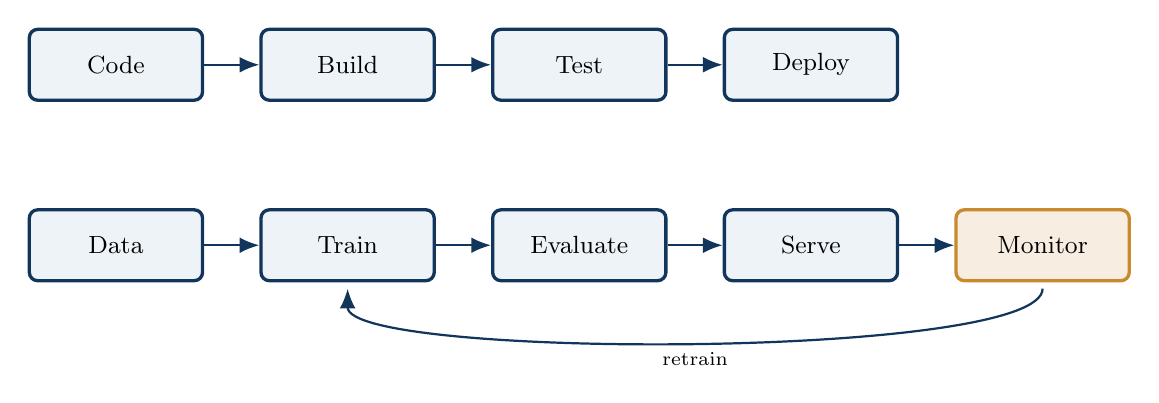
\begin{tikzpicture}[node distance=0.7cm and 0.7cm]
\node[flowbox] (code) {Code};
\node[flowbox, right=of code] (build) {Build};
\node[flowbox, right=of build] (test) {Test};
\node[flowbox, right=of test] (deploy) {Deploy};
\draw[arrow] (code) -- (build);
\draw[arrow] (build) -- (test);
\draw[arrow] (test) -- (deploy);

\node[flowbox, below=1.35cm of code] (data) {Data};
\node[flowbox, right=of data] (train) {Train};
\node[flowbox, right=of train] (eval) {Evaluate};
\node[flowbox, right=of eval] (serve) {Serve};
\node[accentbox, right=of serve] (monitor) {Monitor};
\draw[arrow] (data) -- (train);
\draw[arrow] (train) -- (eval);
\draw[arrow] (eval) -- (serve);
\draw[arrow] (serve) -- (monitor);
\draw[arrow] ($(monitor.south)+(0,-0.08)$)
  .. controls +(0,-0.9) and +(0,-0.9) ..
  node[below, font=\scriptsize] {retrain}
  ($(train.south)+(0,-0.08)$);
\end{tikzpicture}
\vspace{0.5em}
\begin{itemize}
\item The ML lifecycle adds permanent dependence on data quality and drift.
\end{itemize}
\coursefooter
\end{frame}

\begin{frame}{Technology map: analysis and experimentation}
\begin{tabularx}{\textwidth}{>{\bfseries}l X}
Python & General-purpose language used across the whole stack. \\
Jupyter & Interactive environment for exploration, narrative explanation, and teaching labs. \\
pandas & Tabular data manipulation, cleaning, joins, missing-value analysis, and time handling. \\
Matplotlib / seaborn & Static plots for EDA, diagnostics, and teaching. \\
scikit-learn & Classical ML toolkit for preprocessing, pipelines, model training, evaluation, and persistence. \\
\end{tabularx}
\repoactivity{
These appear directly in the notebooks folder and in the fraud modeling workflow.
}
\coursefooter
\end{frame}

\begin{frame}{Technology map: serving and interaction}
\begin{tabularx}{\textwidth}{>{\bfseries}l X}
Flask & Lightweight Python web framework used here to expose prediction and streaming APIs. \\
Streamlit & Rapid framework for interactive data apps and teaching dashboards. \\
River & Online machine learning library for incremental learning and drift-aware workflows. \\
Open-Meteo API & External weather data source used in the streaming demo. \\
JSON / HTTP & The transport layer connecting model services to clients and dashboards. \\
\end{tabularx}
\begin{block}{How they connect}
Flask exposes model or sensor endpoints; Streamlit consumes them for interfaces; River updates models one observation at a time in streaming settings.
\end{block}
\coursefooter
\end{frame}

\begin{frame}{Technology map: packaging and automation}
\begin{tabularx}{\textwidth}{>{\bfseries}l X}
Docker & Packages applications and dependencies into reproducible containers. \\
GitHub Actions & Repository-native automation for tests, builds, and simple CI/CD. \\
Jenkins & Flexible automation server for more customizable pipelines and deployment workflows. \\
Git & Version control for code, and the base coordination layer for team work. \\
\end{tabularx}
\begin{block}{Why students should care}
Without packaging and automation, repeated delivery becomes manual, slow, and error-prone.
\end{block}
\coursefooter
\end{frame}

\begin{frame}{End-to-end view of the course stack}
\centering
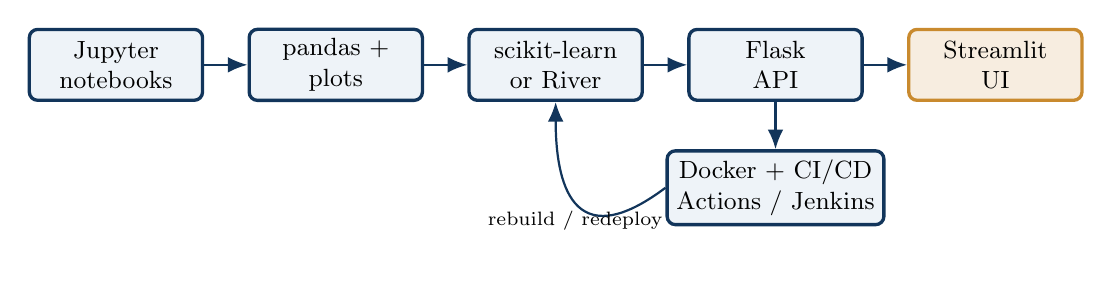
\begin{tikzpicture}[node distance=0.6cm and 0.55cm]
\node[flowbox] (jupyter) {Jupyter\\notebooks};
\node[flowbox, right=of jupyter] (pandas) {pandas +\\plots};
\node[flowbox, right=of pandas] (sk) {scikit-learn\\or River};
\node[flowbox, right=of sk] (flask) {Flask\\API};
\node[accentbox, right=of flask] (st) {Streamlit\\UI};
\node[flowbox, below=of flask] (ops) {Docker + CI/CD\\Actions / Jenkins};
\draw[arrow] (jupyter) -- (pandas);
\draw[arrow] (pandas) -- (sk);
\draw[arrow] (sk) -- (flask);
\draw[arrow] (flask) -- (st);
\draw[arrow] (flask) -- (ops);
\draw[arrow] (ops.west) .. controls +(-1.2,-0.9) and +(0,-1.0) .. node[below, font=\scriptsize] {rebuild / redeploy} (sk.south);
\end{tikzpicture}
\vspace{0.6em}
\begin{itemize}
\item This is the conceptual backbone for almost every class that follows.
\end{itemize}
\coursefooter
\end{frame}

\begin{frame}{Where each technology appears in the repository}
\begin{itemize}
\item `notebooks/`: Jupyter, pandas, scikit-learn, River, and experimentation material.
\item `Class6_model_api.py` and `pasteurization/serving.py`: Flask for prediction and streaming APIs.
\item `streamlit/`: interactive frontends for fraud detection and online learning demos.
\item `tutorials/Docker`, `tutorials/GitHubActions`, `tutorials/Jenkins`: reproducibility and automation material.
\end{itemize}
\coursefooter
\end{frame}

\begin{frame}{When to use which technology}
\begin{tabularx}{\textwidth}{>{\bfseries}l X}
Jupyter & When we are exploring, teaching, comparing ideas, or documenting analysis. \\
scikit-learn & When we need robust tabular ML pipelines and standard offline evaluation. \\
River & When data arrives continuously and the model must update incrementally. \\
Flask & When we need a programmable service endpoint that other systems can call. \\
Streamlit & When we want an interactive dashboard or demo quickly, with low front-end overhead. \\
Docker / CI tools & When we want the system to be repeatable across machines and releases. \\
\end{tabularx}
\coursefooter
\end{frame}

\begin{frame}{Agile AI in practice}
\begin{itemize}
\item Write user stories around decisions, not around algorithms.
\item Deliver thin vertical slices: data ingest, baseline model, API, dashboard, monitor.
\item Prefer fast feedback over premature architectural perfection.
\item Keep scope visible: assumptions, risks, unknown labels, and data quality issues.
\item Treat the first usable model as a learning tool, not as the final product.
\end{itemize}
\coursefooter
\end{frame}

\begin{frame}{Questions students should be able to answer after Class 1}
\begin{itemize}
\item Why is a trained model only one part of a usable system?
\item When would we use Flask rather than Streamlit?
\item Why might River be preferred over scikit-learn in a streaming scenario?
\item What problem does Docker solve that Python alone does not?
\item Why do CI/CD tools matter even in an ML course?
\end{itemize}
\coursefooter
\end{frame}

\begin{frame}{Official technology links}
\readinglist{
\href{https://jupyter.org/install}{Jupyter install guide};\ 
\href{https://pandas.pydata.org/docs/}{pandas documentation};\ 
\href{https://matplotlib.org/stable/}{Matplotlib documentation};\ 
\href{https://scikit-learn.org/stable/}{scikit-learn documentation};\ 
\href{https://flask.palletsprojects.com/en/stable/}{Flask documentation};\ 
\href{https://docs.streamlit.io/}{Streamlit documentation};\ 
\href{https://riverml.xyz/latest/}{River documentation};\ 
\href{https://open-meteo.com/en/docs}{Open-Meteo API docs};\ 
\href{https://docs.docker.com/get-started/}{Docker get started};\ 
\href{https://docs.github.com/en/actions}{GitHub Actions docs};\ 
\href{https://www.jenkins.io/doc/}{Jenkins documentation}.
}
\coursefooter
\end{frame}

\classclosingframe
{\begin{itemize}
\item Data-driven systems must be designed across data, model, interface, delivery, and monitoring concerns.
\item Each technology in the stack solves a different engineering problem, not the same one with different names.
\item The running cases will let us revisit the same lifecycle from multiple technical angles.
\end{itemize}}
{Use this map to explain where your own project sits today and which lifecycle pieces are still missing.}
{Class 2 moves into Python, notebooks, pandas, and exploratory data analysis so we can ground decisions in real datasets before changing features or models.}
{The semester starts with systems thinking so the later technical choices remain connected to a real deployment story.}

\begin{frame}{Foundational readings}
\readinglist{
\href{https://cloud.google.com/architecture/mlops-continuous-delivery-and-automation-pipelines-in-machine-learning}{Google Cloud: MLOps continuous delivery and automation};\ 
\href{https://martinfowler.com/articles/cd4ml.html}{Continuous Delivery for Machine Learning};\ 
\href{https://research.google/pubs/pub46555/}{Hidden Technical Debt in Machine Learning Systems};\ 
\href{https://www.oreilly.com/library/view/designing-machine-learning/9781098107956/}{Designing Machine Learning Systems};\ 
\href{https://www.oreilly.com/library/view/practical-mlops/9781098103002/}{Practical MLOps}.
}
\coursefooter
\end{frame}

\end{document}
